\section{Event and Object Selection}
\label{sec:AN_Selection}

%In this chapter we document the electron, muon, and photon identification and isolation criteria, $E_T^{MET}$ criteria, and provide the results of comparing simulation with data.


\subsection{Event Level Selection}
\label{sec:AN_Selection_EventLevel}

In the final state of the $W\gamma\rightarrow l\nu\gamma$ process we have a lepton, a photon, and a neutrino. Therefore, we select events with exactly one lepton (muon or electron), a photon, both originating from the primary vertex, and with significant missing transverse evergy $E_T^{miss}$. The object selection criteria as well as criteria for the second lepton veto are desribed in Ch.~\ref{sec:AN_ObjectSelection}.

To select events with significant $E_T^{miss}$, we apply a cut on the transverse mass of a $W$~boson of $M_T^W>40$~GeV, where 
\begin{equation}
$M_T^W=\sqrt{(2 \cdot P_T^{l} \cdot E_T^{miss} \cdot (1-\cos{(\phi^{l}-\phi^{miss})}))}$,
\end{equation}
\noindent{where $P_T^l$ is a lepton transverse momentum, $\phi^{l}$ is an azimuthal angle of the lepton momentum, and $\phi^{miss}$ is an azimuthal angle of the missing transverse momentum.}

After that, the significant background from DY+jets$\rightarrow e e \gamma$ in the electron channel remains. This background is caused by one of the electrons misidentified as a photon. Its contribution is the most significant around the invariant mass of the electron-photon system $M_{e\gamma}$ is close to the mass of the $Z$ boson as shown in the $M_{e\gamma}$ distribution (Fig.~\ref{fig:DATAvsMC_Mpholep1}).  To reject this background, we apply $Z$-mass window cut: events with $70$~GeV$<M_{e\gamma}<110$~GeV are rejected. 

Finally, the separation $\Delta R=\sqrt{({\Delta\phi}^2+{\Delta\eta}^2)}$ between the final state lepton and photon is required to be $\Delta R(l,\gamma)>0.7$ to avoid divergence coming from the ISR and FSR contributions and also to enchance the TGC contribution. In case if there are more than one photon in the event passed all selection criteria including the $\Delta R$ cut, the candidate with the hardest photon is selected (one with the highest~$P_T^{\gamma}$). 

\begin{figure}[htb]
  \begin{center}
   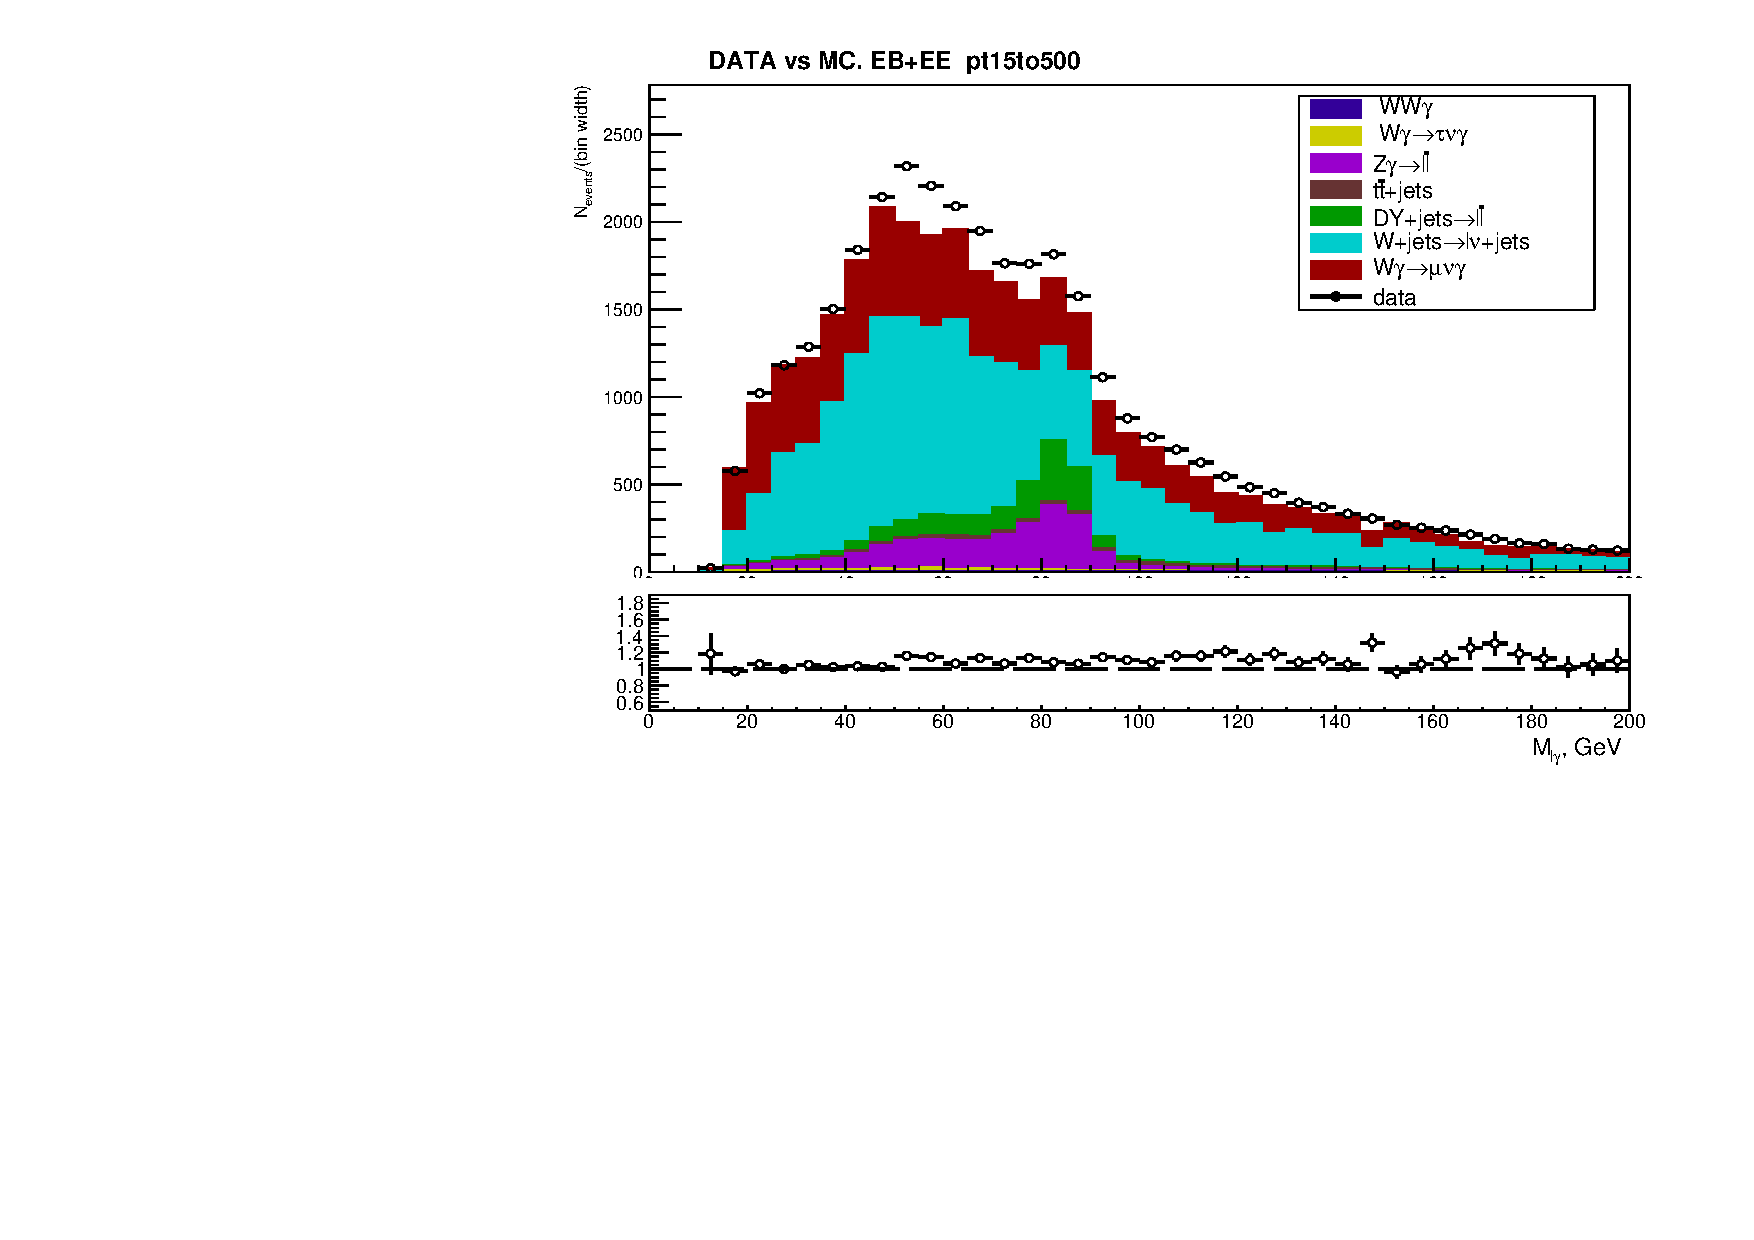
\includegraphics[width=0.5\textwidth]{../figs/figs_v11/MUON_WGamma/PrepareYields/c_TotalDATAvsMC_EtaCommon__Mpholep1_pt15to500_.pdf}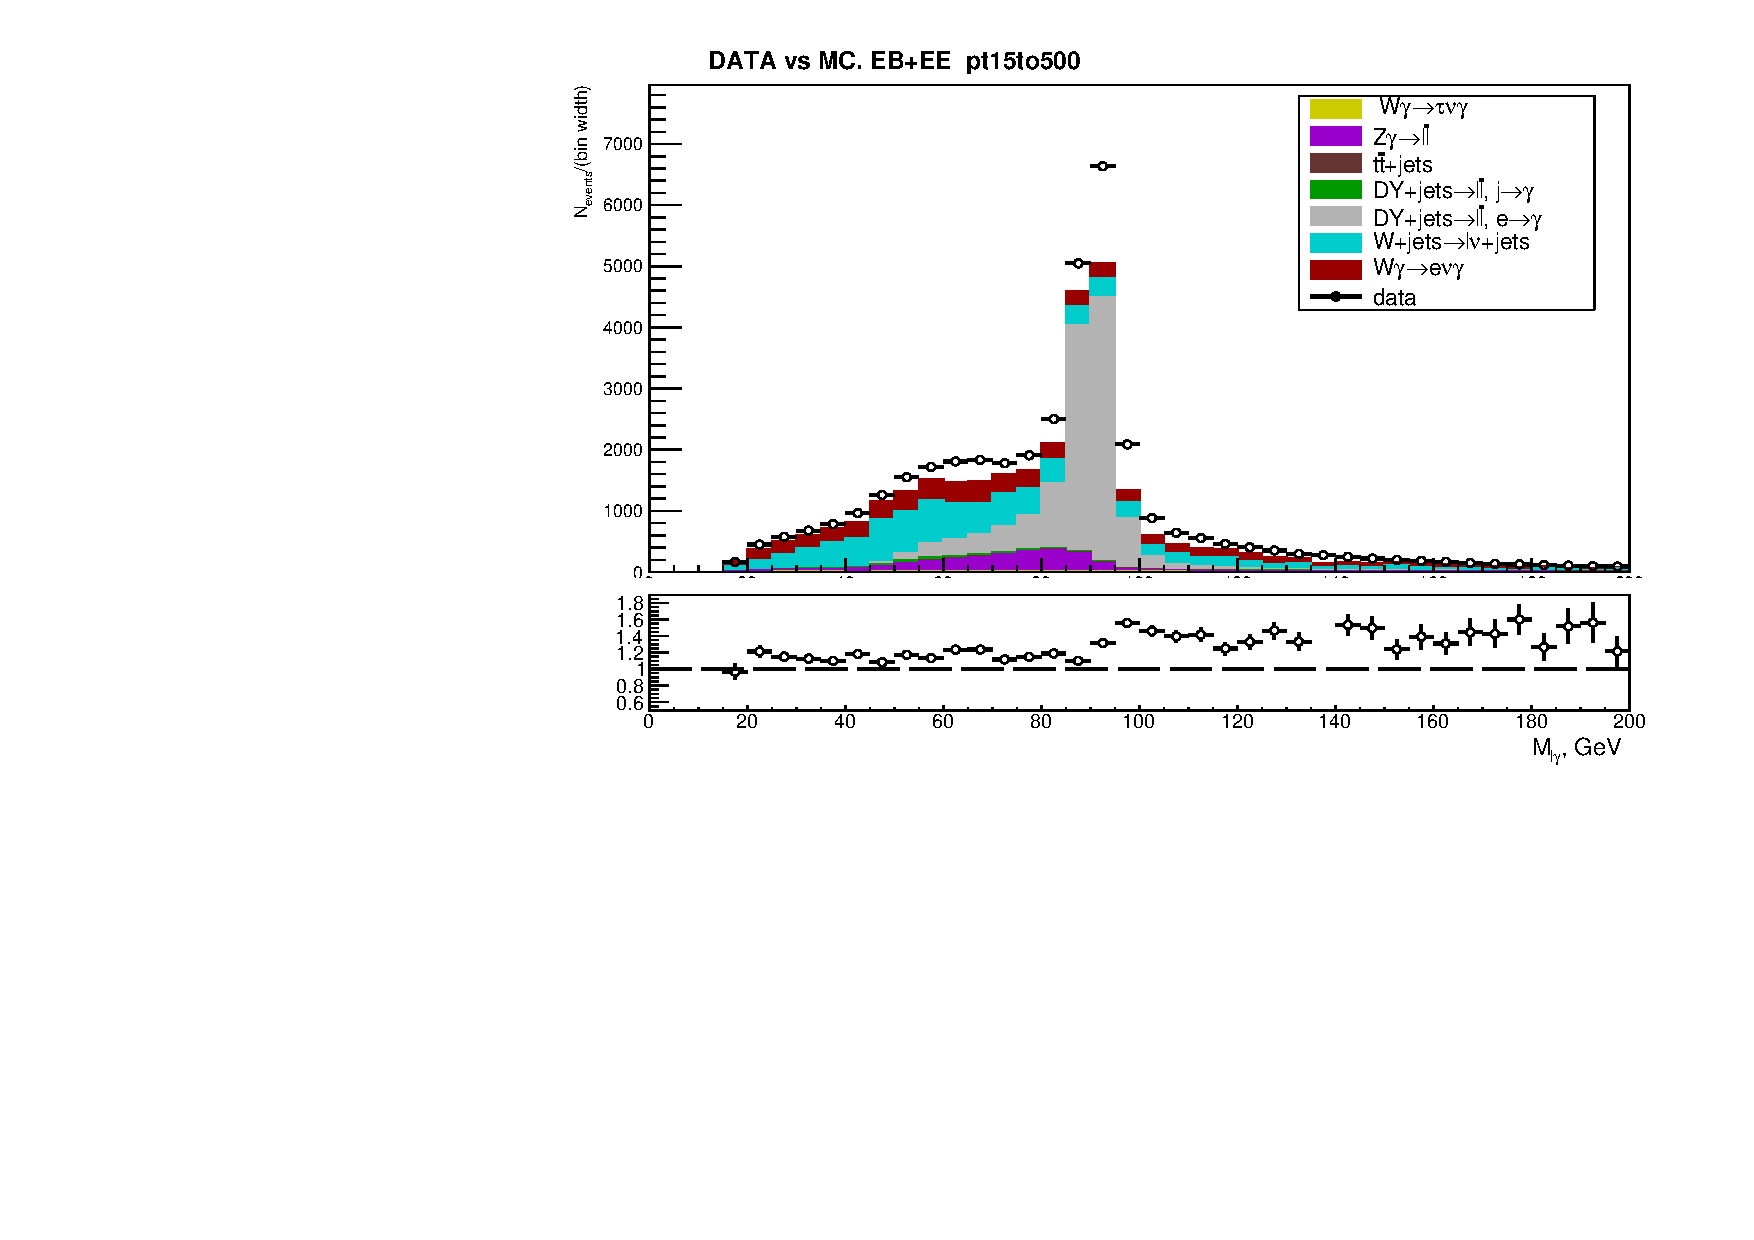
\includegraphics[width=0.5\textwidth]{../figs/figs_v11/ELECTRON_WGamma/PrepareYields/c_TotalDATAvsMC_EtaCommon__Mpholep1PRELIMINARY_FOR_E_TO_GAMMA_WITH_PSV_CUT_pt15to500_.pdf}
  \caption{Data vs MC plots, $M_{l\gamma}$. Left: muon channel, right: electron channel. All selection criteria except $M_{l\gamma}$ cut are applied on these plots. $<P_T^{\gamma}>15$~GeV. Events with $70$~GeV~$<M_{l,\gamma}<110$~GeV are rejected in the electron channel.}
  \label{fig:DATAvsMC_Mpholep1}
  \end{center}
\end{figure}

\subsection{Object Selection}
\label{sec:AN_ObjectSelection}

We select events with muons and photons in the final state for the muon channel and events with electrons and photons in the final state for the electron channel. CMS Particle Object Group (POG) provides all CMS physics measurement groups with their recommendation for object identification~(ID) criteria for any given period of data-taking. Recommendations for~2012 data include two sets of muon~ID criteria: "Tight" and "Loose" and four sets of electron and photon~ID criteria: "Tight", "Medium", "Loose" and "Veto".

For the muon selection, we applied the kinematics cuts of $p_T>25$ GeV and $|\eta|<2.1$ and "Tight"~ID criteria. To reduce backgrounds from the process with two or more muons, like $Z\gamma\rightarrow\mu\mu\gamma$ process, we reject all events that have the second reconstructed muon candidate with $P_T>10$ GeV and $|\eta|<2.4$. 

We consider electrons with $p_T>30$~GeV passing the "Tight" ID criteria and photons with $P_T>15$~GeV passing the modified "Medium" ID criteria. The modification of the photons ID criteria was studied in the $W\gamma\gamma \rightarrow l\nu\gamma\gamma$ measurement~\cite{ref_Wgg8TeV}. 

In addition, electrons and photons must be within the ECal acceptance that is defined in terms of barrel (EB) and endcap (EE) sections with pseudorapidity ranges of $|\eta| < 1.4442$ and $1.566 < |\eta| < 2.5$, respectively. To reject events with two or more final state electrons, events with the second reconstructed electron candidate with $p_T>10$ GeV and satisfying the "Veto"~ID criteria are rejected. %No restrictions on the maximum number of the final state photons are applied, however, . 

Selection criteria are applied consistently on the data sample as well as on all MC samples. The selection efficiency may slightly differ between data and MC. The ratios data and MC efficiencies are called the scale factors. The scale factors for the selection criteria recommended by CMS POG are provided by CMS POG. For the modified photon~ID criteria, the appropriate changes to the POG-recommended scale factors were applied derived by the $W\gamma\gamma$ team~\cite{ref_Wgg8TeV}.

% NEED PLOTS WITH SCALE FACTORS 


\subsection{Selected Events}

%Distributions of $P_T^{\gamma}$ and $M_T^W$ of the selected events are shown in Fig. \ref{fig:DATAvsMC} and \ref{fig:DATAvsMC_WMt}. 
%The is a large discrepancies in all the distributions and therefore the data-driven background estimates are necessary.\\

The PU reweighting is applied on each event in each MC sample. Fig.~\ref{fig:DATAvsMC_nVtx} shows the distribution of the number of vertices for the $Z\gamma$ selected sample in muon channel before (left) and after (right) the PU reweighting of the MC samples. The same procedure of the PU reweighting is applied for the $W\gamma$ selected MC samples.

\begin{figure}[htb]
  \begin{center}
   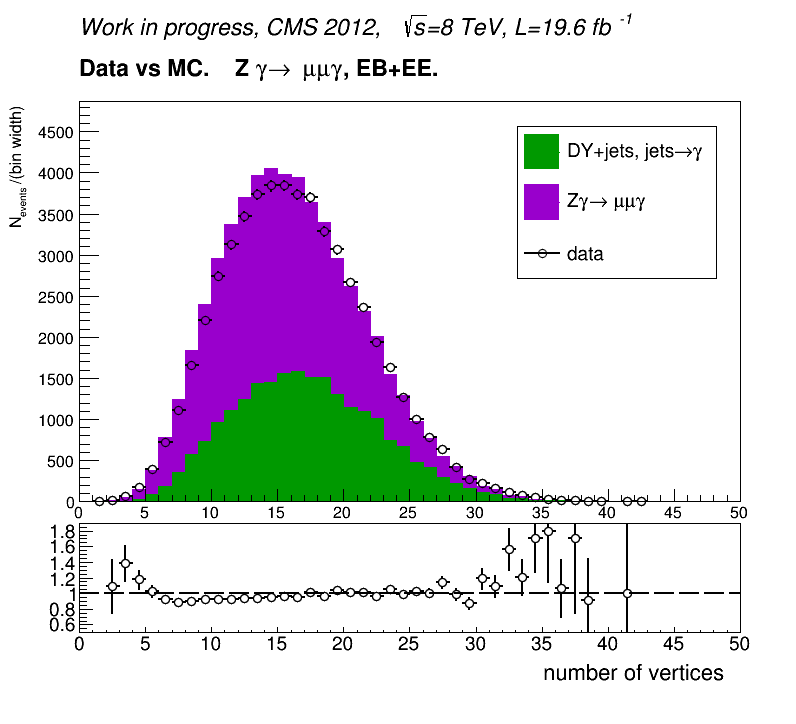
\includegraphics[width=0.45\textwidth]{../figs/figs_v11/MUON_ZGamma/PrepareYields/c_TotalDATAvsMC_EtaCommon__nVtx_noPU.png}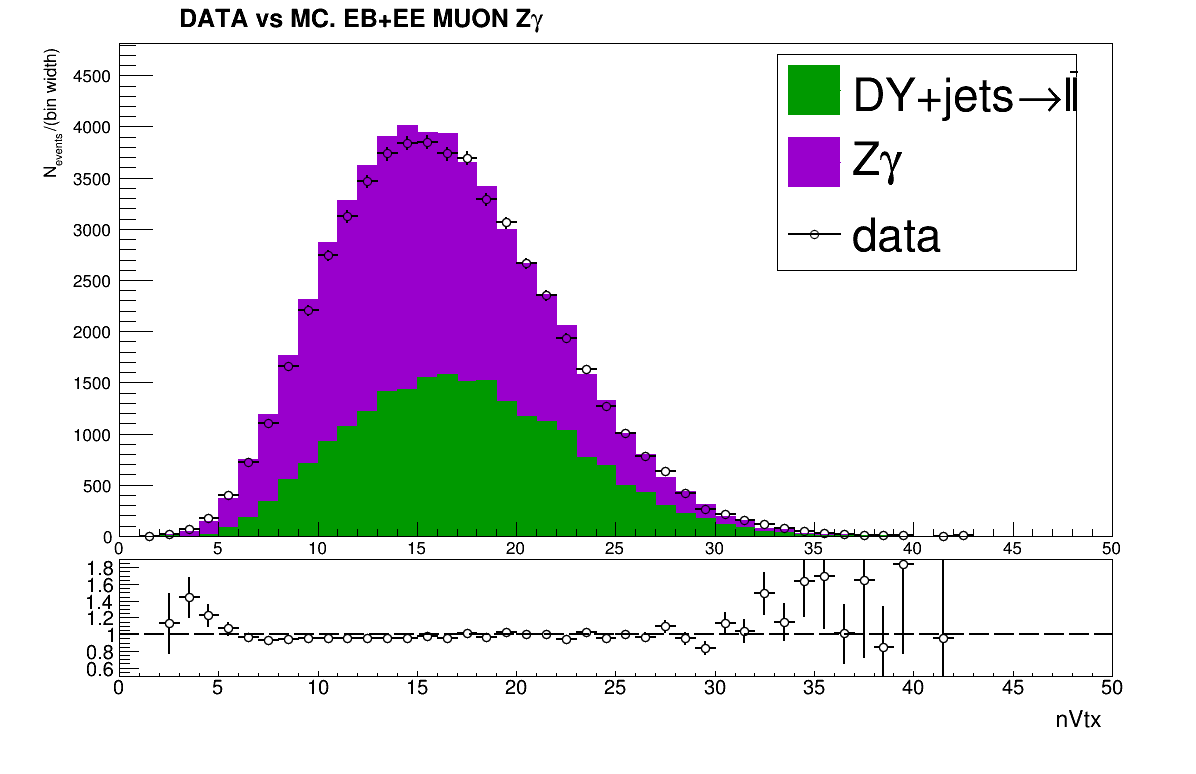
\includegraphics[width=0.45\textwidth]{../figs/figs_v11/MUON_ZGamma/PrepareYields/c_TotalDATAvsMC_EtaCommon__nVtx.png}
  \caption{Number of vertices, data vs MC. $Z\gamma$ selected sample, muon channel. Left: no PU reweighting applied, right: PU reweighting applied. }
  \label{fig:DATAvsMC_nVtx}
  \end{center}
\end{figure}



Our $W$+jets, DY+jets and $t\bar{t}$+jets MC samples partially contain $W\gamma$, $Z\gamma$, and $t\bar{t}\gamma$ events. The overlap was removed from the $W$+jets, DY+jets, and $t\bar{t}$+jets samples relying on their gen-level information. A good data vs MC agreement for the $Z\gamma$ plots in Fig.~\ref{fig:DATAvsMC_nVtx} validates the procedure of the overlap removal.

Distributions of $P_T^{\gamma}$ of the selected events are shown in Fig.~\ref{fig:DATAvsMC}. The are large discrepancies in all the distributions and therefore the data-driven background estimates are necessary.

\begin{figure}[htb]
  \begin{center}
   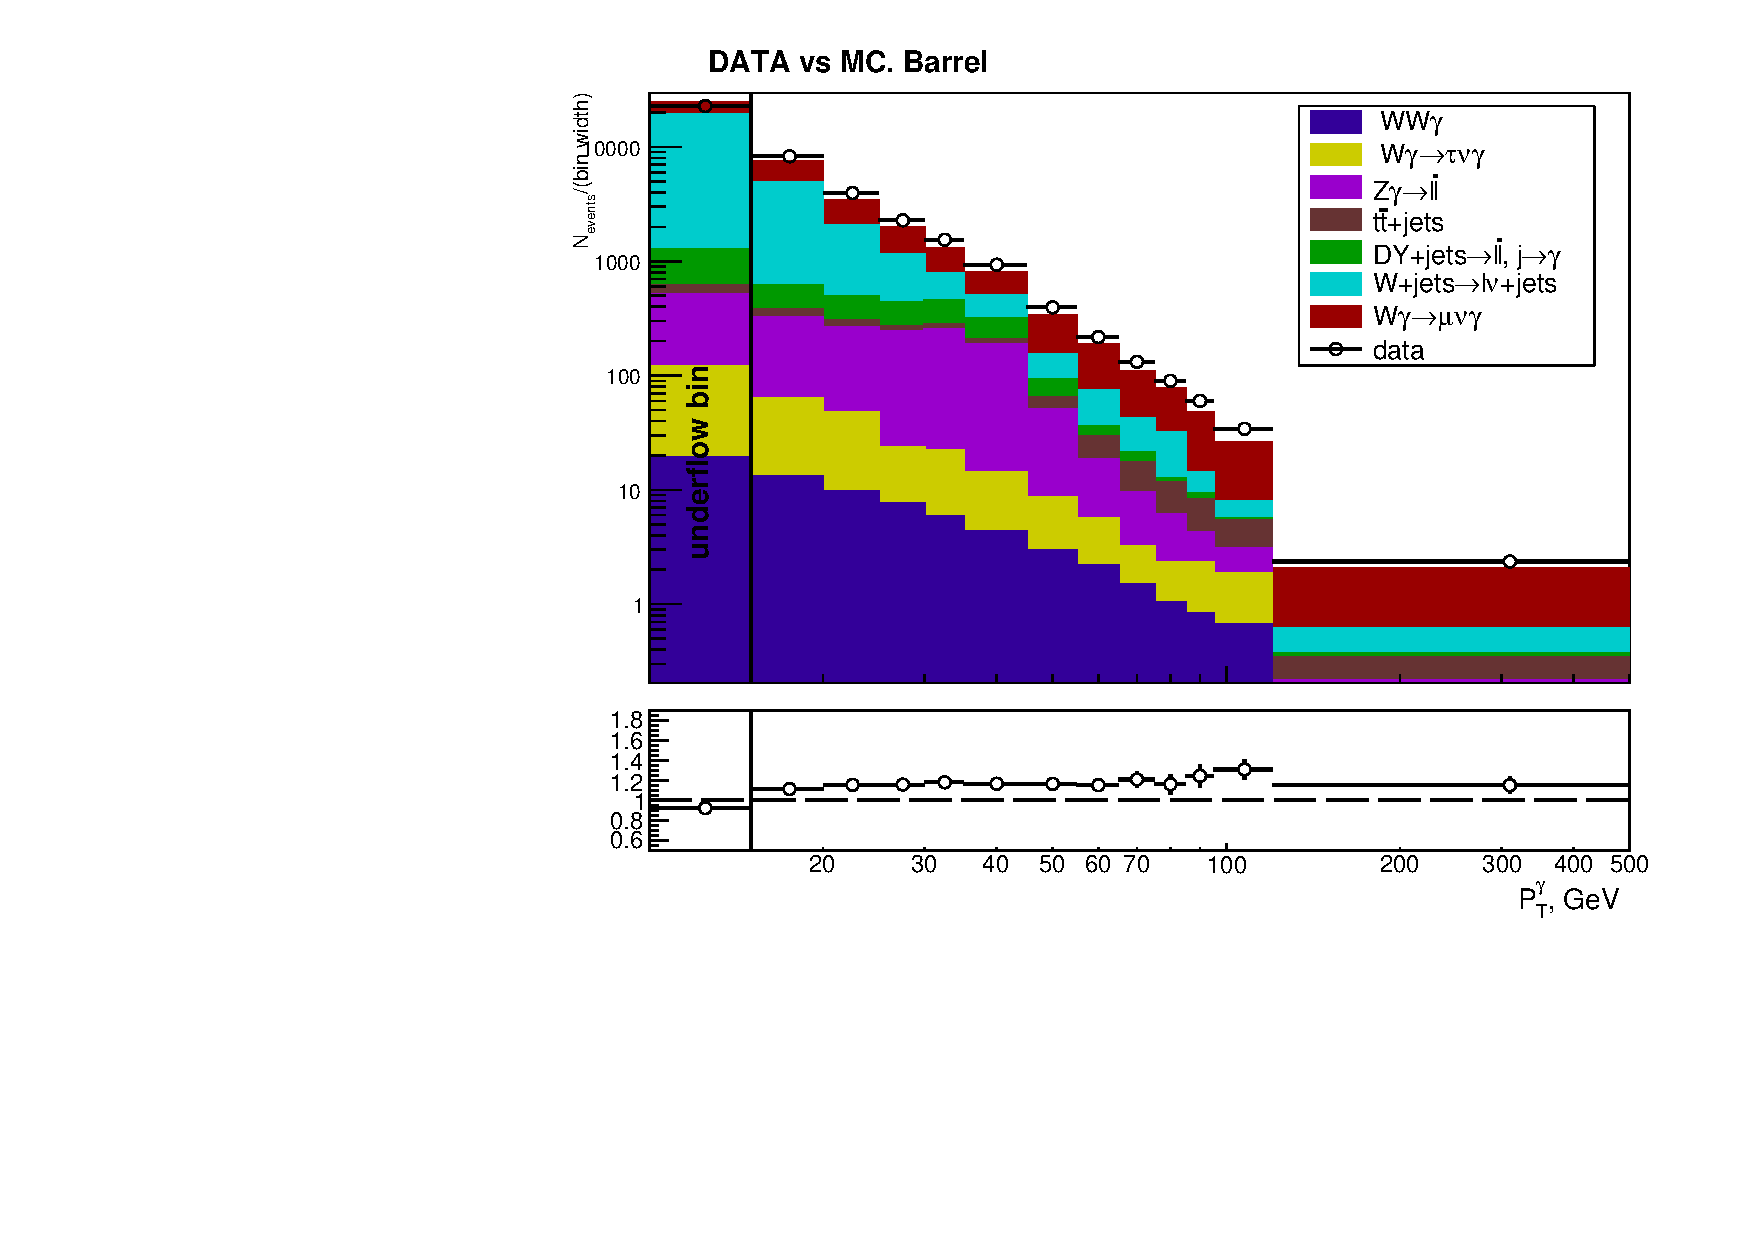
\includegraphics[width=0.45\textwidth]{../figs/figs_v11/MUON_WGamma/PrepareYields/c_TotalDATAvsMC_Barrel__phoEt.pdf}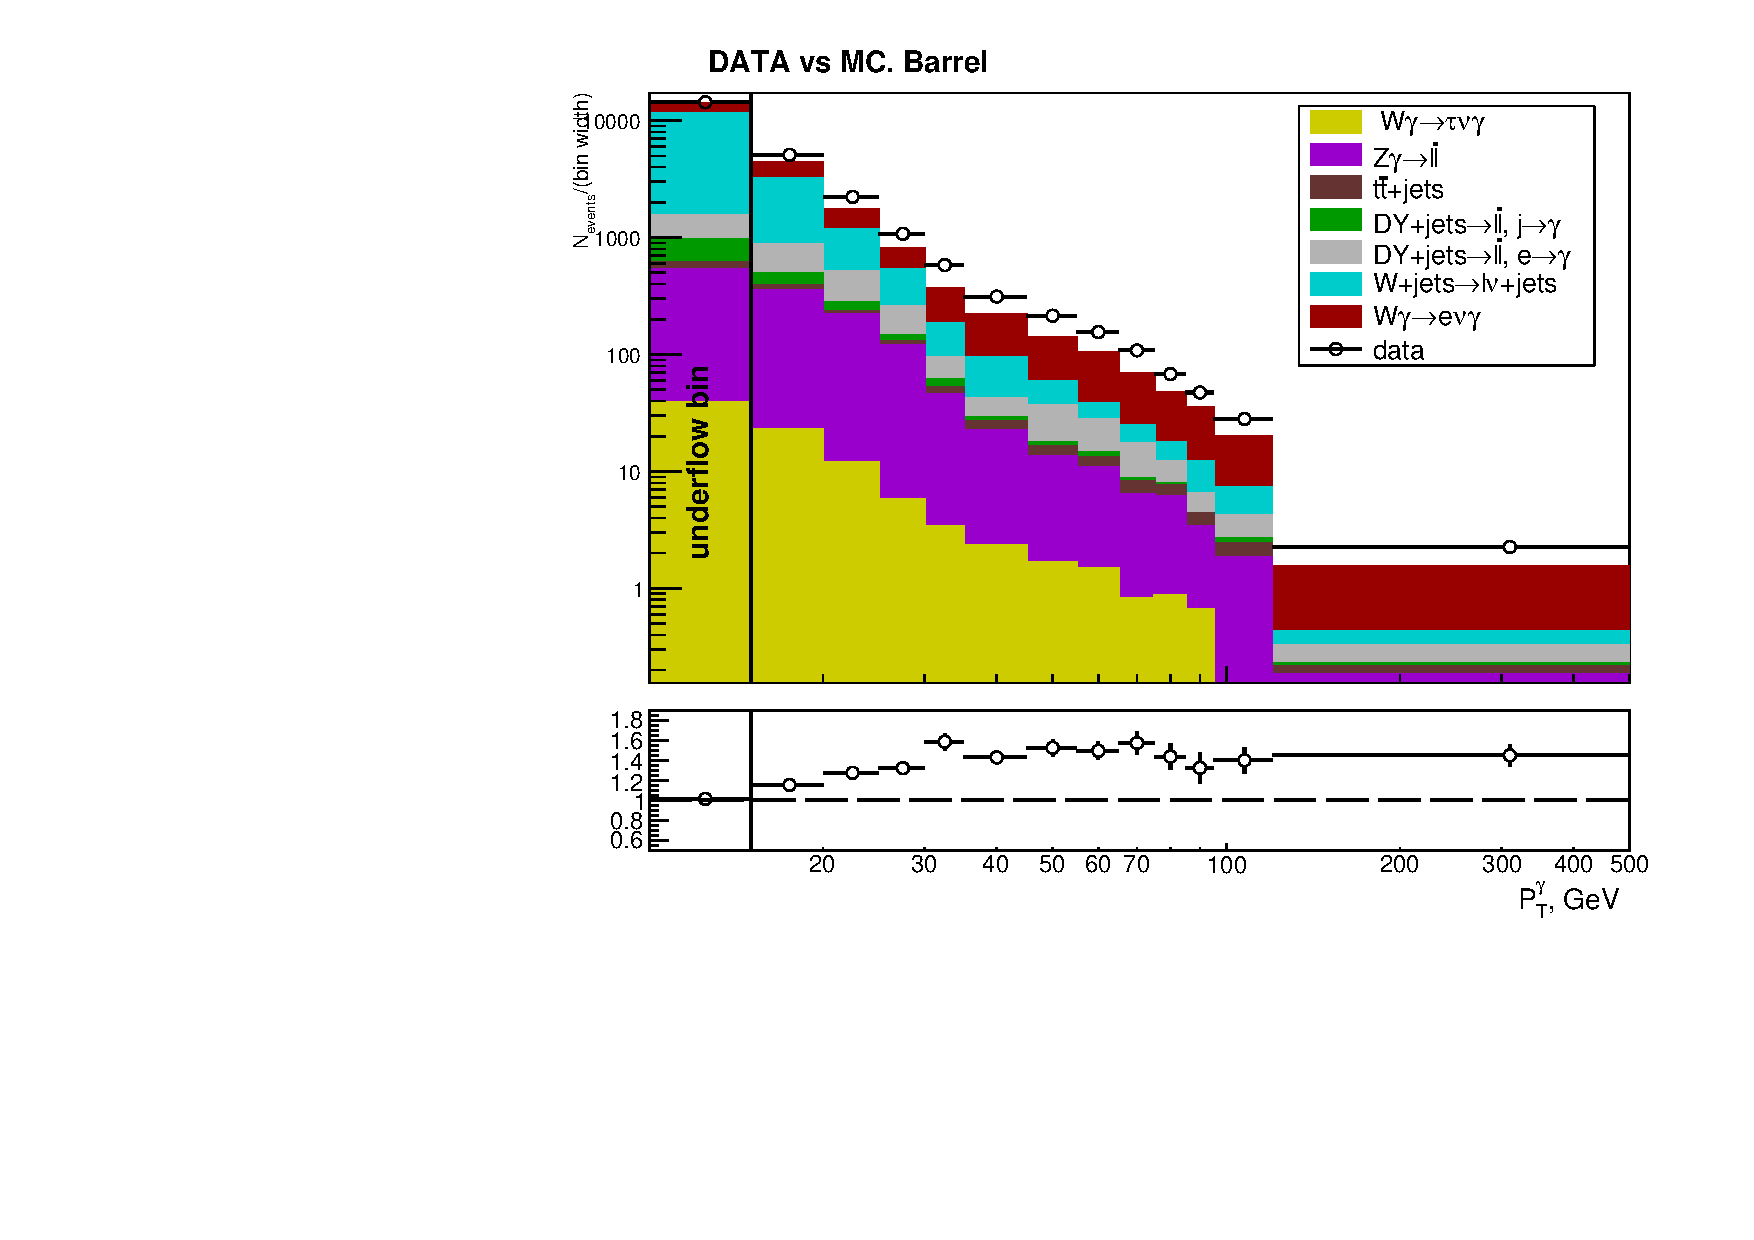
\includegraphics[width=0.45\textwidth]{../figs/figs_v11/ELECTRON_WGamma/PrepareYields/c_TotalDATAvsMC_Barrel__phoEt.pdf}
   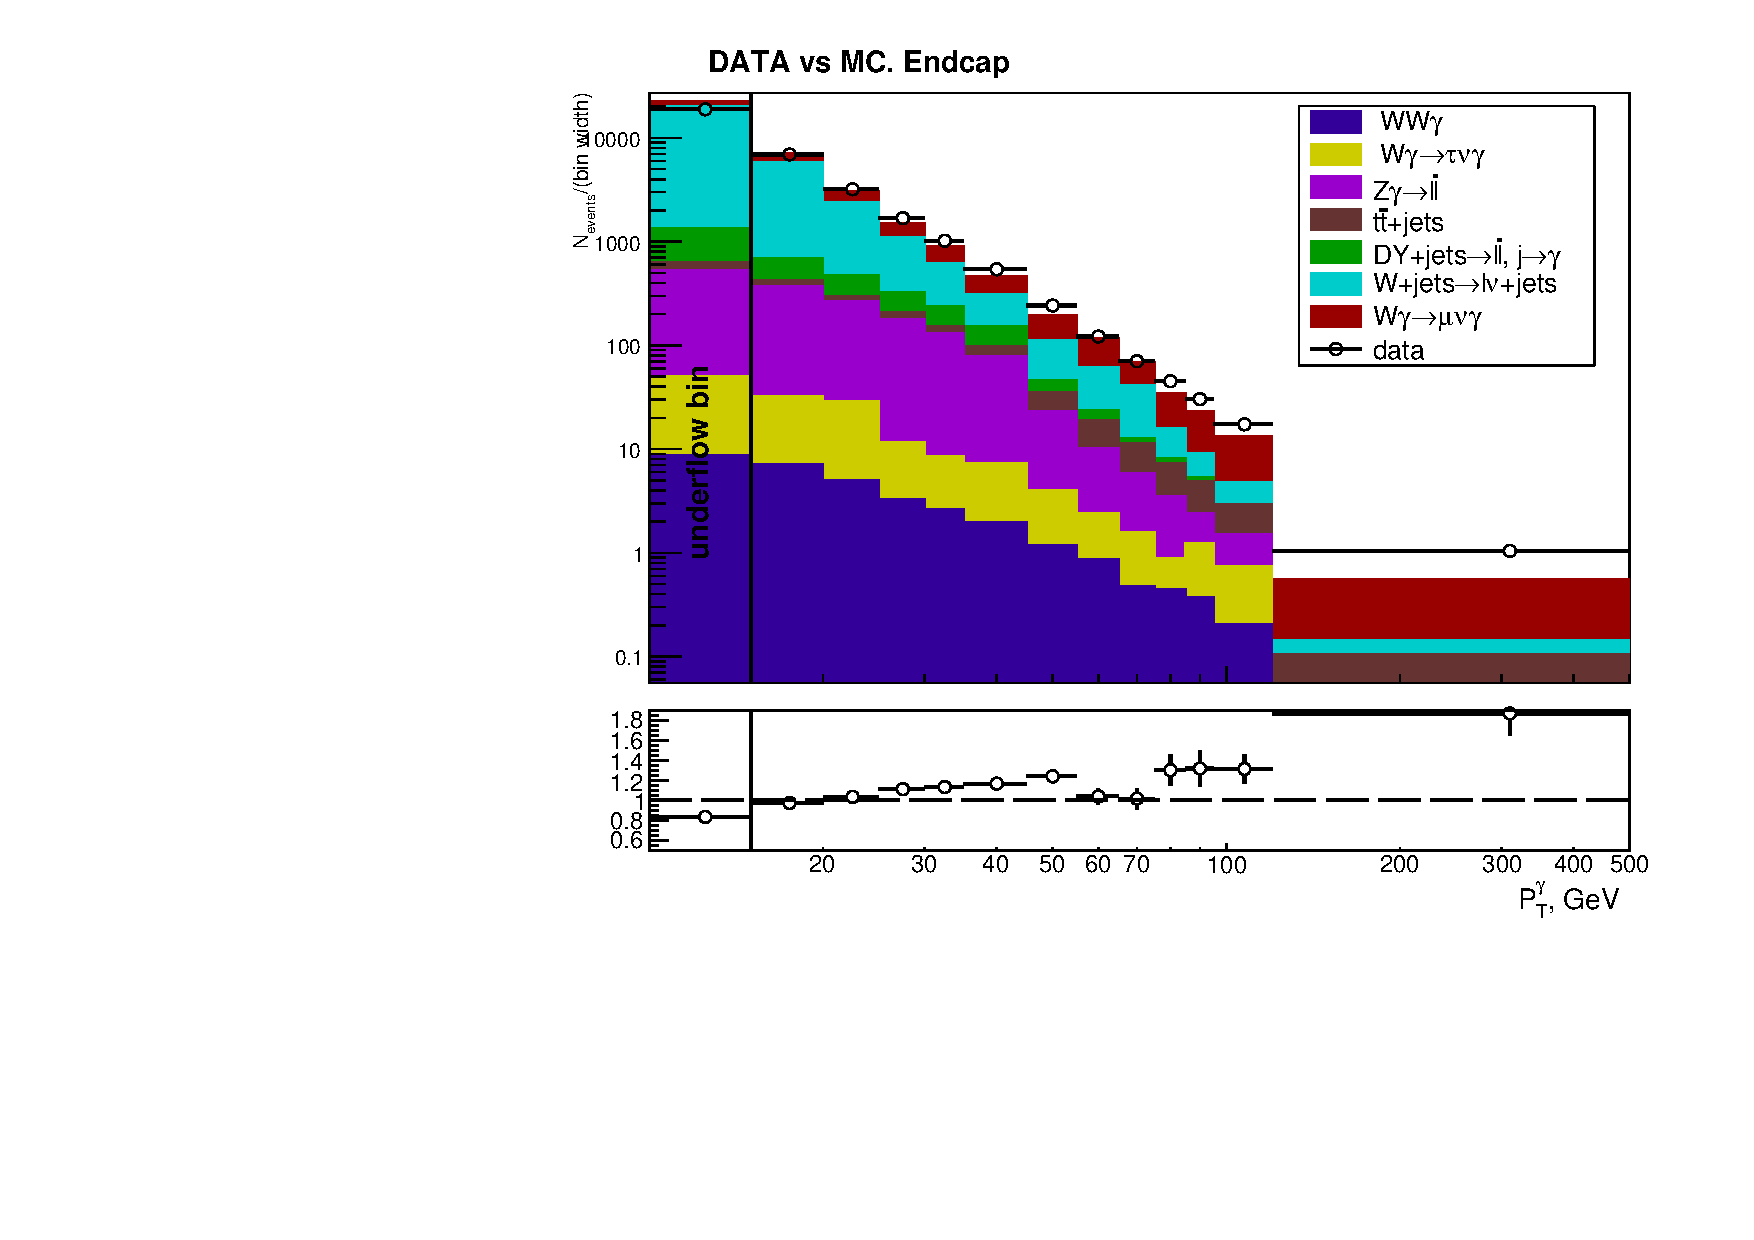
\includegraphics[width=0.45\textwidth]{../figs/figs_v11/MUON_WGamma/PrepareYields/c_TotalDATAvsMC_Endcap__phoEt.pdf}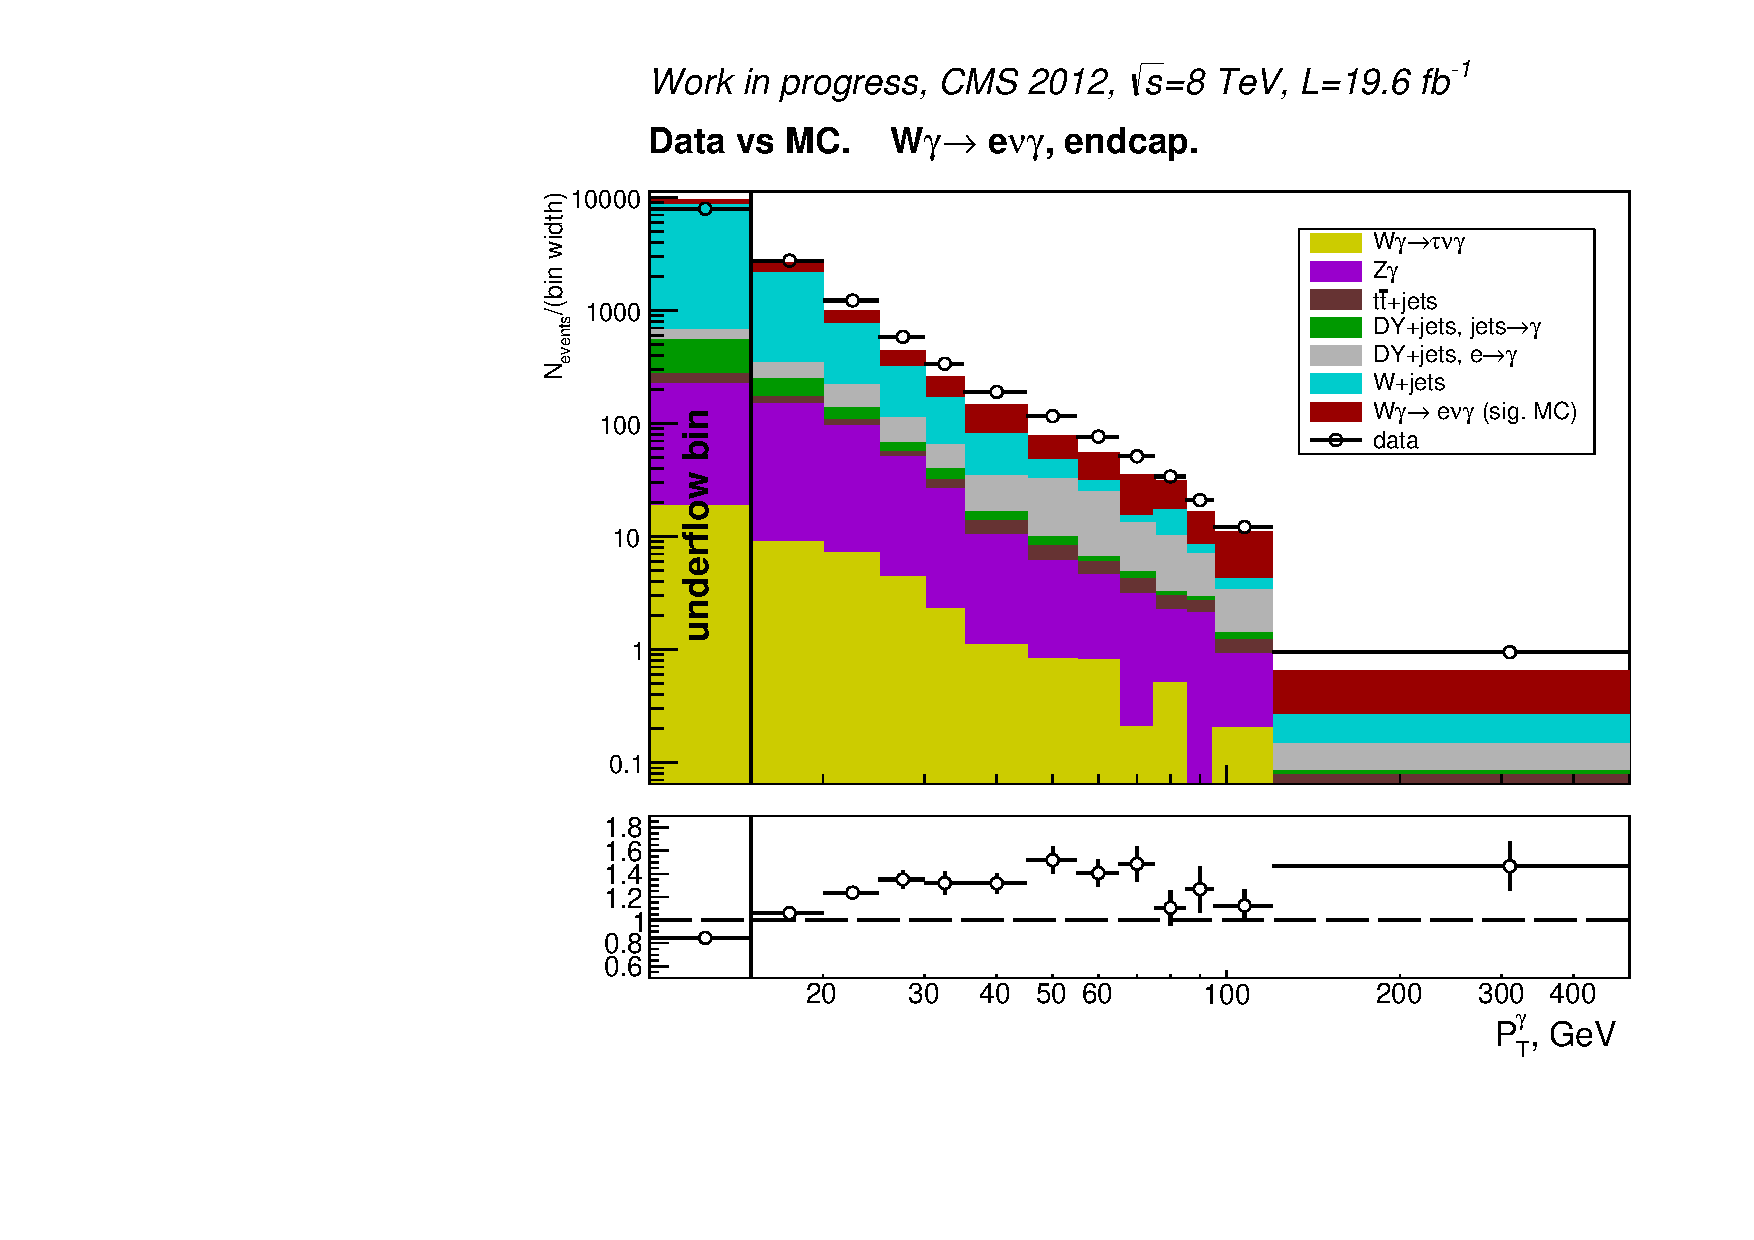
\includegraphics[width=0.45\textwidth]{../figs/figs_v11/ELECTRON_WGamma/PrepareYields/c_TotalDATAvsMC_Endcap__phoEt.pdf}
  \caption{Data vs simulation plots. Left column: muon channel, right column: electron channel. Top to bottom: barrel and endcap photons.}
  \label{fig:DATAvsMC}
  \end{center}
\end{figure}



%\begin{figure}[htb]
%  \begin{center}
%   \includegraphics[width=0.45\textwidth]{figs_v8/MUON_WGamma/PrepareYields/c_TotalDATAvsMC_Barrel__WMtVERY_PRELIMINARY.pdf}\includegraphics[width=0.45\textwidth]{figs_v8/ELECTRON_WGamma/PrepareYields/c_TotalDATAvsMC_Barrel__WMtVERY_PRELIMINARY.pdf}
%   \includegraphics[width=0.45\textwidth]{figs_v8/MUON_WGamma/PrepareYields/c_TotalDATAvsMC_Endcap__WMtVERY_PRELIMINARY.pdf}\includegraphics[width=0.45\textwidth]{figs_v8/ELECTRON_WGamma/PrepareYields/c_TotalDATAvsMC_Endcap__WMtVERY_PRELIMINARY.pdf}
%  \caption{Data vs MC plots, $M_T^W$. Left column - muon channel, right column - electron. Top to bottom: barrel and endcap photons. All selection criteria except $M_T^W$ cut on these plots. $15$~GeV$<P_T^{\gamma}<45$~GeV. The analysis cut of $M_T^W>40$~GeV is selected.}
%  \label{fig:DATAvsMC_WMt}
%  \end{center}
%\end{figure}
